% Level ceiling (grade 6): density handled as "mass of one cubic
% centimetre" via proportionality tables and division; the literal
% formula rho = m/V waits for grade 7 (literal expressions, math g7).
\chapter{La masse volumique~: pourquoi les objets flottent}\label{ch:g6:density-floating}

Dès ta toute première année, une minuscule pièce de monnaie coulait
pendant qu'un grand tronc flottait, et nous avions promis que le
«~pourquoi~» serait un trésor de ce cours. Tu l'as mérité. La clé a
été forgée en deux chapitres --- la \omterm{def:g3:measuring-mass:mass}{masse} pour la matière, le \omterm{def:g6:mass-and-volume:volume}{volume}
pour la place --- et aujourd'hui les deux tournent ensemble dans la
serrure.

\section{La masse d'un centimètre cube}

\begin{example}[Une comparaison enfin honnête]\label{ex:g6:density-floating:fair}
Comparer un tronc entier à une pièce entière n'a jamais été
honnête~: tailles différentes, formes différentes. La compétition
honnête prend des \emph{\omterm{def:g6:mass-and-volume:volume}{volumes} égaux}~: un \omterm{def:g6:mass-and-volume:volume}{centimètre cube} de chaque
concurrent. Un \unit{cm^3} d'eau a une \omterm{def:g3:measuring-mass:mass}{masse} de \qty{1}{g}. Un
\unit{cm^3} de chêne~: environ \qty{0.6}{g}. De pierre~: environ
\qty{2.5}{g}. De fer~: \qty{7.9}{g}. Des places égales, des matières
follement inégales --- voilà le nombre que le jeu de la flottaison
attendait.
\end{example}

\begin{definition}[Masse volumique]\label{def:g6:density-floating:density}
La \emph{masse volumique}\index{masse volumique} d'une substance est
la \omterm{def:g3:measuring-mass:mass}{masse} d'un \omterm{def:g6:mass-and-volume:volume}{centimètre cube} de cette substance, en \omterm{def:g3:measuring-mass:units}{grammes}. La
\omterm{def:g3:measuring-mass:mass}{masse} volumique de l'eau vaut \qty{1}{g} par \unit{cm^3}~; celle du
chêne, environ $0.6$~; celle du fer, $7.9$. Pour trouver une \omterm{def:g3:measuring-mass:mass}{masse}
volumique, aucun instrument nouveau n'est nécessaire~: on mesure la
\omterm{def:g3:measuring-mass:mass}{masse} et le \omterm{def:g6:mass-and-volume:volume}{volume} d'un échantillon, puis on divise --- on partage
les \omterm{def:g3:measuring-mass:units}{grammes} également entre les \omterm{def:g6:mass-and-volume:volume}{centimètres cubes}, et la réponse est
la part de chaque \omterm{def:g6:mass-and-volume:volume}{centimètre cube}.
\end{definition}

\begin{omfigure}
\begin{tikzpicture}[scale=0.85]
  \foreach \x/\name/\m/\c in {0.9/liège/0.2/omMeth,
      3.0/chêne/0.6/omMeth, 5.1/eau/1.0/omDef,
      7.2/pierre/2.5/omExo, 9.3/fer/7.9/omThm} {
    \draw[thick, fill=\c, fill opacity=0.4]
      (\x,0.6) rectangle ++(1.0,1.0);
    \node[above, font=\footnotesize] at (\x+0.5,1.65) {\name};
    \node[below, font=\footnotesize] at (\x+0.5,0.5)
      {$\m$ g};
  }
  \node[below, font=\small] at (5.6,-0.15)
    {cinq cubes égaux d'un centimètre cube --- cinq masses};
\end{tikzpicture}

{\small La compétition honnête~: la même place pour tous, et chaque
substance affiche la \omterm{def:g3:measuring-mass:mass}{masse} qui lui sert de signature.}
\end{omfigure}

\begin{proposition}[La masse volumique est une
signature]\label{prop:g6:density-floating:signature}
La \omterm{def:g6:density-floating:density}{masse volumique} d'une substance pure est la même pour chacun de
ses morceaux, grand ou petit~: un éclat de chêne et une poutre
entière portent tous deux environ \qty{0.6}{g} dans chaque \omterm{def:g6:mass-and-volume:volume}{centimètre
cube}. La \omterm{def:g6:density-floating:density}{masse volumique} identifie donc les substances, comme le font
les \omterm{def:g4:changes-of-state:melting-point}{températures de fusion}~: on mesure la \omterm{def:g3:measuring-mass:mass}{masse} et le \omterm{def:g6:mass-and-volume:volume}{volume} d'un
objet mystérieux, on divise, et on compare avec le tableau --- la
substance avoue souvent sur-le-champ.
\end{proposition}

\begin{method}[Mesurer une masse volumique]\label{met:g6:density-floating:measure}
Pour un caillou --- ou pour une couronne~:
\begin{enumerate}
  \item \omterm{def:g6:measurement-in-science:measuring}{mesurer} sa \omterm{def:g3:measuring-mass:mass}{masse} à la \omterm{def:g3:levers-and-scales:scale}{balance}~: disons \qty{75}{g}~;
  \item \omterm{def:g6:measurement-in-science:measuring}{mesurer} son \omterm{def:g6:mass-and-volume:volume}{volume} par la montée d'eau~: disons
        \qty{30}{cm^3}~;
  \item diviser les \omterm{def:g3:measuring-mass:units}{grammes} par les \omterm{def:g6:mass-and-volume:volume}{centimètres cubes}~:
        $75 \div 30 = 2.5$ --- chaque \omterm{def:g6:mass-and-volume:volume}{centimètre cube} porte
        \qty{2.5}{g}~;
  \item consulter le tableau~: \omterm{def:g6:density-floating:density}{masse volumique} $2.5$ --- notre
        caillou est une pierre ordinaire.
\end{enumerate}
\end{method}

\section{La règle de la flottaison}

\begin{proposition}[Pourquoi les objets flottent]\label{prop:g6:density-floating:rule}
Un objet \omterm{def:g1:floating-and-sinking:words}{flotte} dans l'eau si sa \omterm{def:g6:density-floating:density}{masse volumique} est \emph{plus
petite} que celle de l'eau --- moins de \qty{1}{g} par \omterm{def:g6:mass-and-volume:volume}{centimètre
cube} --- et il \omterm{def:g1:floating-and-sinking:words}{coule} si sa \omterm{def:g6:density-floating:density}{masse volumique} est plus grande. L'eau,
pour ainsi dire, compare l'intrus à elle-même, place pour place~:
plus-léger-que-moi-par-place voyage à la surface~;
plus-lourd-par-place descend. La même règle gouverne tous les
\omterm{def:g3:solids-liquids-gases:liquid}{liquides}, chacun avec sa propre \omterm{def:g6:density-floating:density}{masse volumique} pour arbitre.
\end{proposition}

\begin{omfigure}
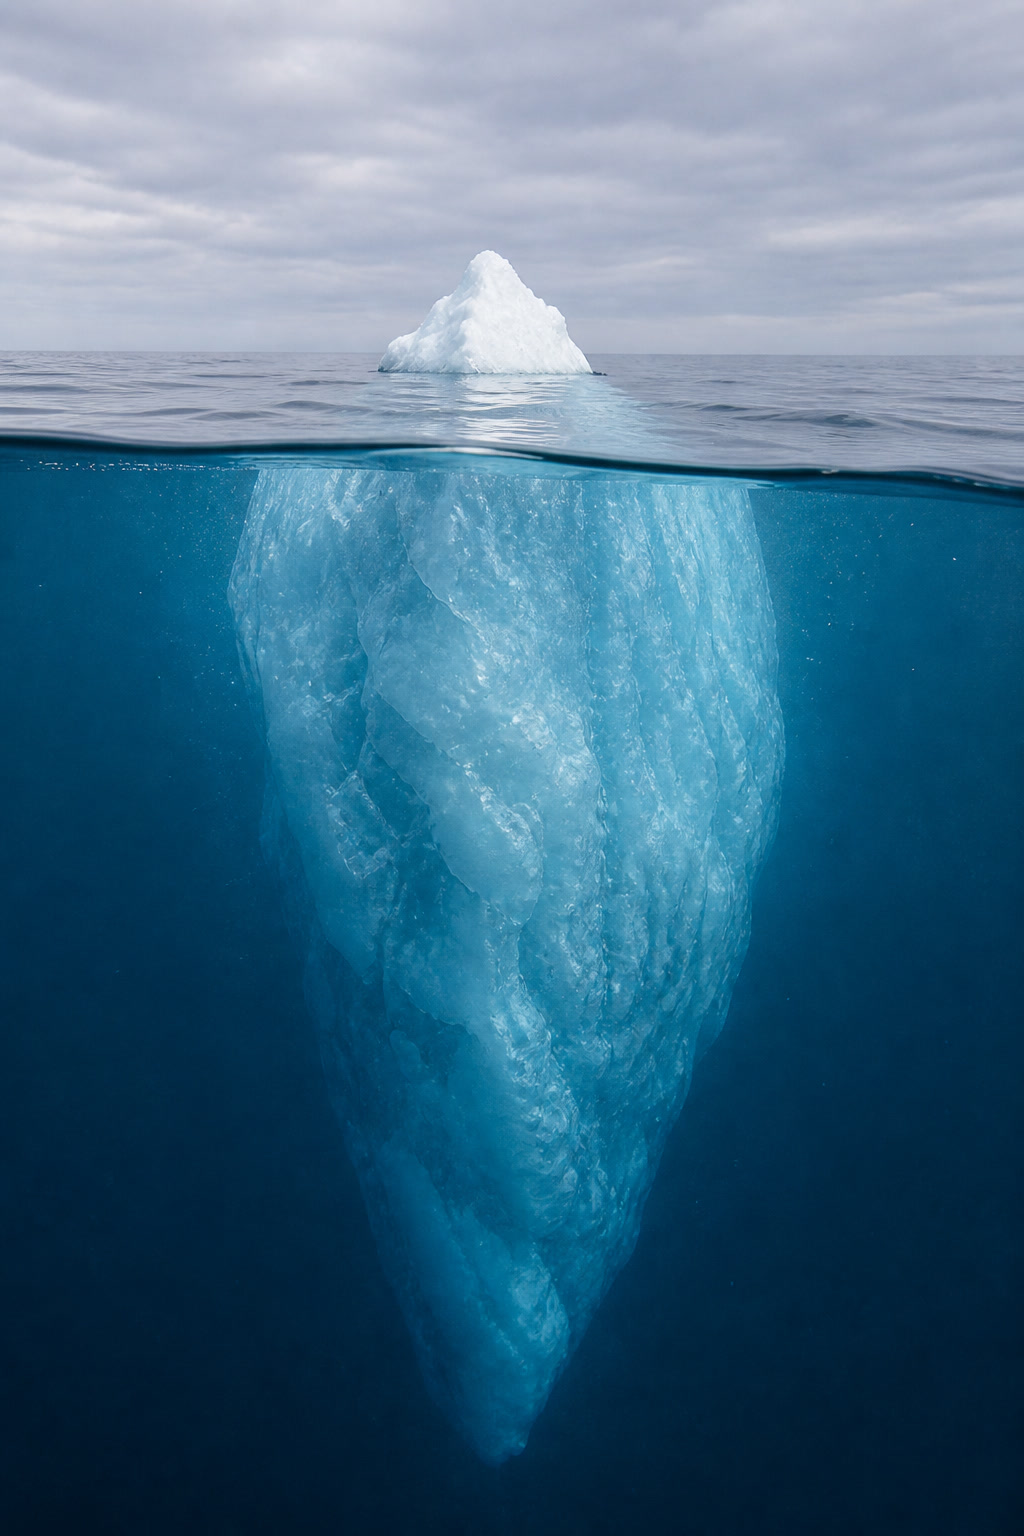
\includegraphics[width=0.4\linewidth]{images/book1/ai/g6-density-iceberg.jpg}

{\small La glace n'est qu'un peu moins dense que l'eau --- un iceberg \omterm{def:g1:floating-and-sinking:words}{flotte} donc très enfoncé, en cachant l'essentiel de sa \omterm{def:g3:measuring-mass:mass}{masse} sous la ligne de flottaison.}
\end{omfigure}

\begin{example}[Six ans d'énigmes, résolues]\label{ex:g6:density-floating:settled}
Le tronc ($0.6$)~: il \omterm{def:g1:floating-and-sinking:words}{flotte}, aussi énorme soit-il --- chacun de ses
\omterm{def:g6:mass-and-volume:volume}{centimètres cubes} fait une offre inférieure à celle de l'eau. La
pièce (en bronze, près de $9$)~: elle \omterm{def:g1:floating-and-sinking:words}{coule}, aussi petite
soit-elle. Le canard en plastique, le bouchon de liège, le crayon~:
au-dessous de $1$, tous flotteurs. La glace, à $0.9$ --- le \omterm{def:g3:solids-liquids-gases:solid}{solide}
gonflé de l'eau elle-même --- \omterm{def:g1:floating-and-sinking:words}{flotte} sur son propre \omterm{def:g3:solids-liquids-gases:liquid}{liquide} d'un
cheveu, ce qui explique que les étangs portent des couvercles et que
les icebergs naviguent. Et le bateau en pâte à modeler~? Façonné en
barquette, le colis \emph{bateau-plus-air} contient beaucoup d'\omterm{def:g2:air-around-us:air}{air}
par \omterm{def:g6:measurement-in-science:measuring}{unité} de place~: la \omterm{def:g6:density-floating:density}{masse volumique} du colis passe au-dessous de
$1$, et sur les quais, la même astuce lance des navires d'acier de
dix mille tonnes.
\end{example}

\begin{omfigure}
\begin{tikzpicture}[scale=0.85]
  \draw[thick] (0.8,0) -- (0.8,3.4) (4.0,0) -- (4.0,3.4)
    (0.8,0) -- (4.0,0);
  \fill[omMeth, opacity=0.35] (0.8,2.2) rectangle (4.0,3.0);
  \node[font=\footnotesize] at (2.4,2.6) {huile~: $0.9$};
  \fill[omDef, opacity=0.3] (0.8,1.1) rectangle (4.0,2.2);
  \node[font=\footnotesize] at (2.4,1.65) {eau~: $1.0$};
  \fill[omThm, opacity=0.3] (0.8,0.05) rectangle (4.0,1.1);
  \node[font=\footnotesize] at (2.4,0.55) {miel~: $1.4$};
  \node[below, font=\small] at (2.4,-0.3)
    {la tour de liquides~: le plus dense en bas};
  \draw[thick] (7.2,0) -- (7.2,3.4) (11.0,0) -- (11.0,3.4)
    (7.2,0) -- (11.0,0);
  \fill[omDef, opacity=0.3] (7.2,0.05) rectangle (11.0,2.6);
  \draw[thick, fill=white]
    (8.3,2.35) -- (9.9,2.35) -- (9.6,2.95) -- (8.6,2.95) -- cycle;
  \draw[thick, fill=white, fill opacity=0.7]
    (8.0,2.35) -- (10.2,2.35) -- (9.5,1.0) -- (8.7,1.0) -- cycle;
  \node[font=\footnotesize] at (9.1,1.85) {glace~: $0.9$};
  \node[below, font=\small] at (9.1,-0.3)
    {l'iceberg~: neuf dixièmes sous la ligne de flottaison};
\end{tikzpicture}

{\small L'écriture de la \omterm{def:g6:density-floating:density}{masse volumique}~: les \omterm{def:g3:solids-liquids-gases:liquid}{liquides} s'empilent du
plus dense en bas, et la glace à $0.9$ ne laisse qu'un dixième
d'elle-même au-dessus de l'eau.}
\end{omfigure}

\begin{example}[La tour de liquides]\label{ex:g6:density-floating:tower}
Verse du miel, puis de l'eau colorée à l'encre, puis de l'huile
doucement le long de la paroi d'un grand verre~: trois couches, le
miel ($1.4$) au fond, l'huile ($0.9$) au sommet, refusant de mélanger
leurs rangs. Fais-y tomber des invités~: un grain de raisin ($1.05$)
traverse l'huile, traverse l'eau, et se pose sur le miel --- plus
dense que deux étages, plus léger que le troisième. La tour est la
règle de la flottaison jouée au théâtre.
\end{example}

\begin{remark}[Lire l'iceberg]\label{rem:g6:density-floating:iceberg}
Le $0.9$ de la glace face au $1.0$ de l'eau fait plus que faire
\omterm{def:g1:floating-and-sinking:words}{flotter} l'iceberg~: il fixe la ligne de flottaison. Neuf dixièmes du
\omterm{def:g6:mass-and-volume:volume}{volume} d'un iceberg voyagent \emph{sous} la surface --- la fameuse
\omterm{def:g3:measuring-mass:mass}{masse} cachée qui a coulé de fiers navires. \emph{Pourquoi}, exactement,
la fraction immergée est égale au rapport des \omterm{def:g6:density-floating:density}{masses volumiques} est
une magnifique loi du savant antique de la baignoire lui-même,
honnêtement démontrée dans le \omterm{def:g6:mass-and-volume:volume}{volume} du lycée~; le tableau des \omterm{def:g6:density-floating:density}{masses
volumiques} en murmure déjà la réponse.
\end{remark}

\section{La couronne, enfin}

\begin{example}[Archimède clôt l'affaire]\label{ex:g6:density-floating:crown}
Achevons maintenant l'histoire commencée deux chapitres plus tôt. La
\omterm{def:g3:measuring-mass:mass}{masse} de la couronne~: facile, la \omterm{def:g3:levers-and-scales:scale}{balance} la donne. Son \omterm{def:g6:mass-and-volume:volume}{volume}~:
impossible pour un chef-d'œuvre biscornu --- jusqu'à ce que la leçon
de la baignoire livre la méthode de la montée d'eau. La \omterm{def:g3:measuring-mass:mass}{masse} divisée
par le \omterm{def:g6:mass-and-volume:volume}{volume}~: la \emph{\omterm{def:g6:density-floating:density}{masse volumique}} de la couronne --- et une
\omterm{def:g6:density-floating:density}{masse volumique} est une signature. L'or pur signe $19.3$~; l'argent
signe $10.5$~; un mélange secret signe quelque part entre les deux.
La légende dit que la couronne de l'orfèvre avoua une \omterm{def:g6:density-floating:density}{masse volumique}
bien inférieure à celle de l'or, et que la fraude fut démasquée sans
une égratignure sur la couronne. Le problème du week-end te remet ses
nombres.
\end{example}

\section{Exercices}

\begin{exercise}[$\star$]\label{exo:g6:density-floating:1}
Qu'est-ce que la \omterm{def:g6:density-floating:density}{masse volumique} d'une substance~? Donne celle de
l'eau, et énonce la règle de la flottaison.
\end{exercise}

\begin{exercise}[$\star$]\label{exo:g6:density-floating:2}
Prédis «~\omterm{def:g1:floating-and-sinking:words}{flotte}~» ou «~\omterm{def:g1:floating-and-sinking:words}{coule}~» dans l'eau~: le chêne ($0.6$)~; \ la
pierre ($2.5$)~; \ le liège ($0.2$)~; \ le fer ($7.9$)~; \ la glace
($0.9$).
\end{exercise}

\begin{exercise}[$\star$]\label{exo:g6:density-floating:3}
Un bloc a une \omterm{def:g3:measuring-mass:mass}{masse} de \qty{120}{g} et un \omterm{def:g6:mass-and-volume:volume}{volume} de \qty{80}{cm^3}.
Trouve sa \omterm{def:g6:density-floating:density}{masse volumique}. Flotte-t-il ou coule-t-il~?
\end{exercise}

\begin{exercise}[$\star$]\label{exo:g6:density-floating:4}
Un morceau mystérieux~: \omterm{def:g3:measuring-mass:mass}{masse} \qty{158}{g}, montée dans l'éprouvette
\qty{20}{cm^3}. Sa \omterm{def:g6:density-floating:density}{masse volumique} --- et, d'après les nombres du
chapitre, sa substance probable~?
\end{exercise}

\begin{exercise}[$\star$]\label{exo:g6:density-floating:5}
Pourquoi la \omterm{def:g6:density-floating:density}{masse volumique} d'un éclat de chêne est-elle la même que
celle d'une poutre de chêne entière~? À quoi cette propriété
sert-elle~?
\end{exercise}

\begin{exercise}[$\star$]\label{exo:g6:density-floating:6}
Dans la tour de \omterm{def:g3:solids-liquids-gases:liquid}{liquides}, pourquoi le miel est-il au fond et l'huile
au sommet~? Où s'immobilise un grain de raisin de \omterm{def:g6:density-floating:density}{masse volumique}
$1.05$~?
\end{exercise}

\begin{exercise}[$\star$]\label{exo:g6:density-floating:7}
La glace \omterm{def:g1:floating-and-sinking:words}{flotte} sur l'eau --- pourquoi est-ce étrange pour un \omterm{def:g3:solids-liquids-gases:solid}{solide},
et quelle vieille proposition sur l'eau qui \omterm{def:g2:ice-water-steam:meltfreeze}{gèle} explique le $0.9$~?
\end{exercise}

\begin{exercise}[$\star$]\label{exo:g6:density-floating:8}
Le grand tronc et la petite pièce de ta première année~: donne la
réponse finale et complète, avec les nombres du chapitre.
\end{exercise}

\begin{exercise}[$\star\star$]\label{exo:g6:density-floating:9}
Un \omterm{def:g6:mass-and-volume:volume}{litre} d'un certain \omterm{def:g3:solids-liquids-gases:liquid}{liquide} a une \omterm{def:g3:measuring-mass:mass}{masse} de \qty{800}{g}. Quelle est
sa \omterm{def:g6:density-floating:density}{masse volumique} en \omterm{def:g3:measuring-mass:units}{grammes} par \omterm{def:g6:mass-and-volume:volume}{centimètre cube}~? Un glaçon
($0.9$) y flottera-t-il ou y coulera-t-il~?
\end{exercise}

\begin{exercise}[$\star\star$]\label{exo:g6:density-floating:10}
L'acier signe $7.9$, et pourtant les navires en acier flottent.
Résous le paradoxe avec l'idée du colis de
\cref{ex:g6:density-floating:settled} --- que contient le
colis-navire en plus de l'acier, et que doit valoir sa \omterm{def:g6:density-floating:density}{masse
volumique} d'ensemble~? À quel moment un navire percé cesse-t-il de
satisfaire la règle~?
\end{exercise}

\begin{exercise}[$\star\star$]\label{exo:g6:density-floating:11}
L'eau de mer est un peu plus dense que l'eau douce --- environ
$1.03$. Explique pourquoi les nageurs flottent nettement mieux en
mer, et prédis ce qui arrive à la ligne de flottaison d'un navire
qui passe de la mer salée à un fleuve d'eau douce.
\end{exercise}

\begin{exercise}[$\star\star\star$]\label{exo:g6:density-floating:12}
Une sphère métallique creuse \omterm{def:g1:floating-and-sinking:words}{flotte} exactement à moitié immergée dans
l'eau. Raisonne pour trouver la \omterm{def:g6:density-floating:density}{masse volumique} du \emph{colis-sphère
entier} (coque métallique plus l'\omterm{def:g2:air-around-us:air}{air} à l'intérieur). Puis argumente
dans quel sens elle se déplace si de l'eau s'infiltre lentement à
l'intérieur, et à quel moment elle se met à \omterm{def:g1:floating-and-sinking:words}{couler} --- la règle et le
colis, main dans la main.
\end{exercise}

\section{Problème~: la couronne du roi}

\begin{problem}[{Problème du week-end --- l'affaire de la couronne du
roi, rouverte avec tes instruments~; le procès de l'orfèvre, résolu
par une division}]\label{pb:g6:density-floating:1}
Rouvre la plus célèbre affaire de fraude de l'Antiquité avec des
nombres modernes. Signatures~: l'or $19.3$, l'argent $10.5$ (en
\omterm{def:g3:measuring-mass:units}{grammes} par \omterm{def:g6:mass-and-volume:volume}{centimètre cube}).

\medskip\noindent\textbf{Partie I --- les preuves.}
Le roi a remis à l'orfèvre \qty{1930}{g} d'or pur. La couronne
achevée, sur la \omterm{def:g3:levers-and-scales:scale}{balance}~: \qty{1930}{g} exactement.
\begin{enumerate}
  \item La \omterm{def:g3:measuring-mass:mass}{masse} correspond parfaitement. Pourquoi cela ne prouve-t-il
        rien à soi seul au sujet de la fraude~? (Qu'aurait pu faire
        l'orfèvre tout en obtenant la même \omterm{def:g3:measuring-mass:mass}{masse}~?)
  \item Quel \omterm{def:g6:mass-and-volume:volume}{volume} \qty{1930}{g} d'\emph{or pur} devraient-ils
        occuper~? (Partage les \omterm{def:g3:measuring-mass:units}{grammes}~: combien de \omterm{def:g6:mass-and-volume:volume}{centimètres
        cubes} à \qty{19.3}{g} chacun~?)
  \item Archimède plonge la couronne dans un récipient plein à ras
        bord et recueille le débordement~: \qty{130}{cm^3}. Quel est
        le vrai \omterm{def:g6:mass-and-volume:volume}{volume} de la couronne~?
  \item Compare les deux \omterm{def:g6:mass-and-volume:volume}{volumes}. Que crie déjà cette comparaison~?
\end{enumerate}

\medskip\noindent\textbf{Partie II --- la signature.}
\begin{enumerate}[resume]
  \item Calcule la \omterm{def:g6:density-floating:density}{masse volumique} de la couronne à partir de sa
        \omterm{def:g3:measuring-mass:mass}{masse} et de son \omterm{def:g6:mass-and-volume:volume}{volume} mesuré (une décimale suffit).
  \item Aligne les trois signatures~: l'or, la couronne, l'argent.
        Où tombe la couronne~?
  \item Explique au roi, en une phrase, pourquoi la couronne ne peut
        pas être en or pur.
  \item L'orfèvre proteste~: «~La \omterm{def:g3:levers-and-scales:scale}{balance} s'est peut-être trompée~!~»
        Accorde-lui une erreur généreuse de \qty{30}{g} dans un sens
        ou dans l'autre. Une \omterm{def:g3:measuring-mass:mass}{masse} comprise entre \qty{1900}{g} et
        \qty{1960}{g} sauve-t-elle une couronne d'or pur de \omterm{def:g6:mass-and-volume:volume}{volume}
        \qty{130}{cm^3}~? (Contrôle l'intervalle des \omterm{def:g6:density-floating:density}{masses
        volumiques}.)
\end{enumerate}

\medskip\noindent\textbf{Partie III --- combien a-t-il volé~?}
Supposons que l'orfèvre ait gardé une partie de l'or et l'ait
remplacée, \omterm{def:g3:measuring-mass:units}{gramme} pour \omterm{def:g3:measuring-mass:units}{gramme}, par de l'argent.
\begin{enumerate}[resume]
  \item Pourquoi remplacer de l'or par de l'argent, \omterm{def:g3:measuring-mass:units}{gramme} pour
        \omterm{def:g3:measuring-mass:units}{gramme}, garde-t-il la \omterm{def:g3:measuring-mass:mass}{masse} exacte tout en \emph{gonflant}
        le \omterm{def:g6:mass-and-volume:volume}{volume}~?
  \item Teste une hypothèse~: une couronne de \qty{965}{g} d'or $+$
        \qty{965}{g} d'argent. \omterm{def:g6:mass-and-volume:volume}{Volume} de la part d'or~? De la part
        d'argent~? (Une décimale.)
  \item Fais le total du \omterm{def:g6:mass-and-volume:volume}{volume} de cette couronne hypothétique, et
        juge l'hypothèse face aux \qty{130}{cm^3} mesurés~: trop
        d'argent, ou trop peu~?
  \item La cour attend une phrase de verdict~: dis ce qui a été
        prouvé sans doute possible (or pur ou non), quelle a été la
        méthode, et pourquoi la couronne n'a jamais eu besoin d'être
        abîmée --- le véritable triomphe d'Archimède.
\end{enumerate}
\end{problem}
